\documentclass{standalone}
% \usepackage[a4paper,landscape,inner=40pt]{geometry}
\usepackage{tikz}
\usepackage{pgfplots}
\pgfplotsset{compat=newest}
\usepackage{mathptmx}
\usepackage{varwidth}
\usepackage{enumitem}
\usetikzlibrary{calc,patterns,decorations.pathmorphing,decorations.markings,matrix,fit,decorations.pathreplacing,automata,positioning,shapes,chains,spy}
\usetikzlibrary{intersections,through,backgrounds,arrows.meta}
\usetikzlibrary{shadows,fadings}
% \usepackage[active,tightpage,pdftex]{preview}
% \PreviewEnvironment{tikzpicture}
\definecolor{inputColor}{HTML}{833EC3}
\definecolor{provisionColor}{HTML}{D23AD0}
\definecolor{recomGenColor}{HTML}{2B6BD1}
\definecolor{ingredientsColor}{HTML}{0BBFCE}
\definecolor{overridingColor}{HTML}{58BD1B}
\definecolor{basicFPGenColor}{HTML}{FED02F}
\definecolor{optimalFPGenColor}{HTML}{F45E30}
\definecolor{finalFPGenColor}{HTML}{E81E49}
\definecolor{optimalFPColor}{HTML}{833EC3}
\pgfdeclarelayer{client}
\pgfdeclarelayer{server}
\pgfdeclarelayer{phaseA}
\pgfdeclarelayer{phaseB}
\pgfsetlayers{client,server,phaseA,phaseB,main}
\begin{document}
  \large
  % \scriptsize
  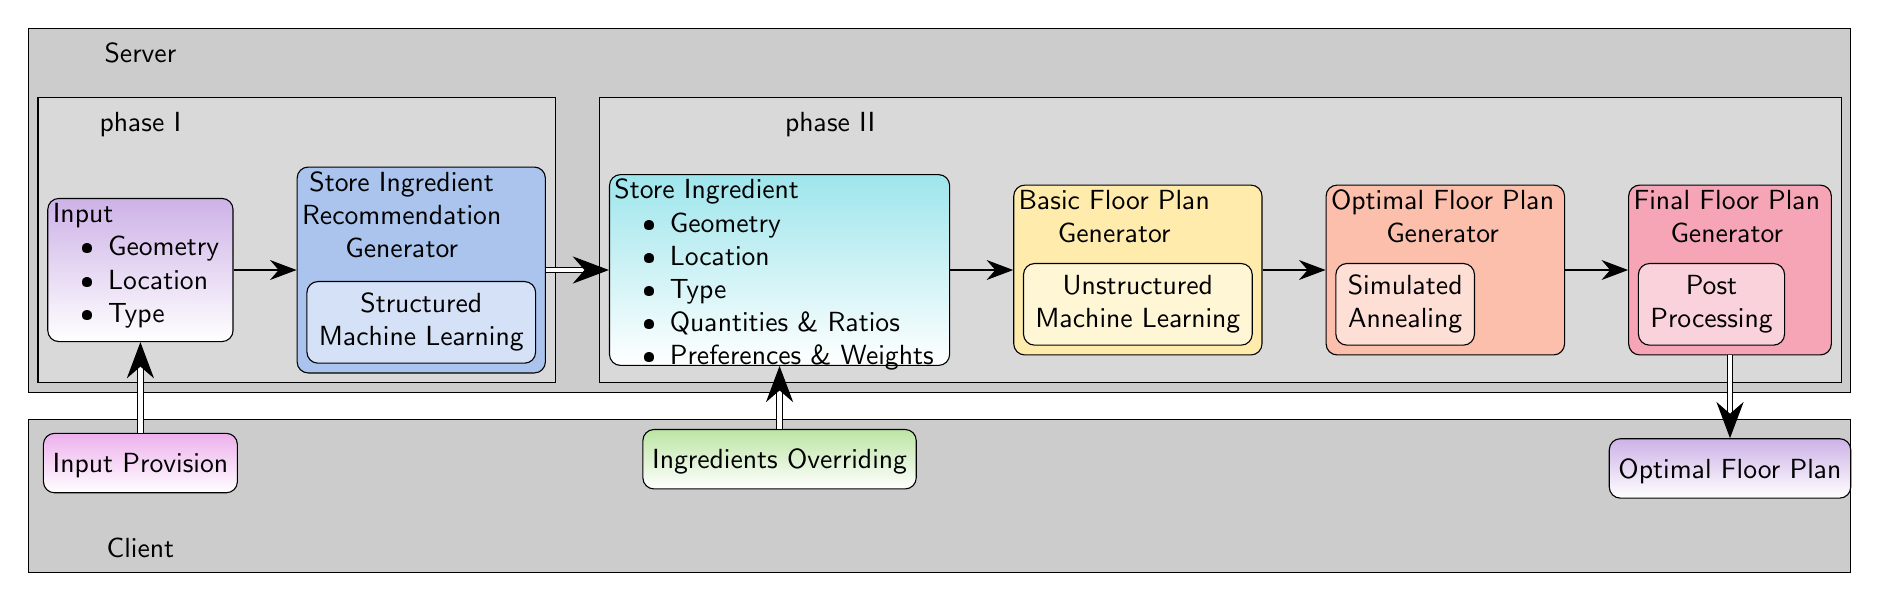
\begin{tikzpicture}[%
      >={Stealth[scale=2.0]},align=center,every node/.style={font=\sffamily}]
    \tikzstyle{typetag}=[inner sep=1ex,anchor=west]
    \tikzstyle{title}=[draw=none,inner sep=0pt,anchor=north west,outer sep=2pt]
    \tikzstyle{mymatrix}=[matrix of nodes,nodes=typetag,row sep=1em]
    \tikzstyle{state}=[text centered,node distance=0.8cm,%
      rectangle,rounded corners,fill=white,draw=black,%
      minimum width=1.0cm,minimum height=0.45cm]
    % All state styles
    \tikzstyle{input}=[state,minimum width=14ex,minimum height=10ex,top color=inputColor!40]
    \tikzstyle{provision}=[state,top color=provisionColor!40]
    \tikzstyle{structuredML}=[state,fill=recomGenColor!20]
    \tikzstyle{recomGen}=[state,minimum height=6ex,fill=recomGenColor!40]
    \tikzstyle{ingredients}=[state,minimum width=27ex,minimum height=14ex,top color=ingredientsColor!40]
    \tikzstyle{overriding}=[state,top color=overridingColor!40]
    \tikzstyle{unstructuredML}=[state,fill=basicFPGenColor!20]
    \tikzstyle{basicFPGen}=[state,fill=basicFPGenColor!40]
    \tikzstyle{simAnn}=[state,fill=optimalFPGenColor!20]
    \tikzstyle{optimalFPGen}=[state,minimum width=18ex,fill=optimalFPGenColor!40]
    \tikzstyle{postProc}=[state,fill=finalFPGenColor!20]
    \tikzstyle{finalFPGen}=[state,minimum width=15ex,fill=finalFPGenColor!40]
    \tikzstyle{optimalFP}=[state,top color=optimalFPColor!40]
    \tikzstyle{client}=[draw,fill=gray!40]
    \tikzstyle{phaseA}=[draw,fill=gray!30]
    \tikzstyle{phaseB}=[draw,fill=gray!30]
    \tikzstyle{server}=[draw,fill=gray!40]
    % States
    \matrix[mymatrix,input] (input) {
      |[title]|\phantom{aaaaaaaaaaa}\\
    };
    \matrix[mymatrix,provision,below=of input,yshift=-1em] (provision) {
      |[title]|Input Provision\\
    };
    \matrix[mymatrix,recomGen,right=of input] (recomGen) {
      |[title]|\phantom{aaaaaaaaaaa}\\
      \node [structuredML] {Structured\\Machine Learning};\\
    };
    \matrix[mymatrix,ingredients,right=of recomGen] (ingredients) {
      |[title]|\phantom{aaaaaaaaaaa}\\
    };
    \matrix[mymatrix,overriding,below=of ingredients] (overriding) {
      |[title]|Ingredients Overriding\\
    };
    \matrix[mymatrix,basicFPGen,right=of ingredients] (basicFPGen) {
      |[title]|\phantom{aaaaaaaaaaa}\\
      \node [unstructuredML] {Unstructured\\Machine Learning};\\
    };
    \matrix[mymatrix,optimalFPGen,right=of basicFPGen] (optimalFPGen) {
      |[title]|\phantom{aaaaaaaaaaa}\\
      \node [simAnn] {Simulated\\Annealing};\\
    };
    \matrix[mymatrix,finalFPGen,right=of optimalFPGen] (finalFPGen) {
      |[title]|\phantom{aaaaaaaaaaa}\\
      \node [postProc] {Post\\Processing};\\
    };
    \matrix[mymatrix,optimalFP,below=of finalFPGen,yshift=-0.25cm] (optimalFP) {
      |[title]|Optimal Floor Plan\\
    };
    % Text
    \node[title] () at (input.north west) {%
      \makebox{%
        \begin{varwidth}{\linewidth}
          Input
          \begin{itemize}[noitemsep,topsep=0pt,parsep=0pt,partopsep=0pt,leftmargin=2em]
          \item Geometry
          \item Location
          \item Type
          \end{itemize}
      \end{varwidth}}%
    };
    \node[title] () at (recomGen.north west)
         {Store Ingredient\\Recommendation\\Generator};
    \node[title] () at (ingredients.north west) {%
      \makebox{%
        \begin{varwidth}{\linewidth}
          Store Ingredient
          \begin{itemize}[noitemsep,topsep=0pt,parsep=0pt,partopsep=0pt,leftmargin=2em]
          \item Geometry
          \item Location
          \item Type
          \item Quantities \& Ratios
          \item Preferences \& Weights
          \end{itemize}
      \end{varwidth}}%
    };
    \node[title] () at (basicFPGen.north west) {Basic Floor Plan\\Generator};
    \node[title] () at (optimalFPGen.north west){Optimal Floor Plan\\Generator};
    \node[title] () at (finalFPGen.north west) {Final Floor Plan\\Generator};
    % Edges
    \draw [->,double equal sign distance] (provision) -- (input);
    \draw [->] (input) -- (recomGen);
    \draw [->,double equal sign distance] (recomGen) -- (ingredients);
    \draw [->] (ingredients) -- (basicFPGen);
    \draw [->,double equal sign distance] (overriding) -- (ingredients);
    \draw [->] (basicFPGen) -- (optimalFPGen);
    \draw [->] (optimalFPGen) -- (finalFPGen);
    \draw [->,double equal sign distance] (finalFPGen) -- (optimalFP);
    % Layers
    % Phase I
    \node (phaseATitle) [title,above=of input,yshift=-0.3cm] {phase I};
    \begin{pgfonlayer}{phaseA}
      \node (phaseA) [phaseA,fit=(input)(recomGen)(phaseATitle)] {};
    \end{pgfonlayer}{phaseA}
    % Phase II
    \node (phaseBTitle) at (ingredients.center|-phaseATitle.north)
    [title] {phase II};
    \begin{pgfonlayer}{phaseB}
      \node (phaseB) [phaseB,fit=(ingredients)(basicFPGen)(optimalFPGen)(finalFPGen)(phaseBTitle)(ingredients.east|-recomGen.south)] {};
    \end{pgfonlayer}{phaseB}
    % Server
    \node (serverTitle) [title,above=of phaseATitle,yshift=-0.5cm] {Server};
    \begin{pgfonlayer}{server}
      \node (server) [server,fit=(phaseA)(phaseB)(serverTitle)] {};
    \end{pgfonlayer}{server}
    % Client
    \node (clientTitle) [title,below=of provision,yshift=0.5cm] {Client};
    \begin{pgfonlayer}{client}
      \node (client)
      [client,fit=(provision)(overriding)(clientTitle)(phaseA.west|-provision.center)(phaseB.east|-overriding.center)] {};
    \end{pgfonlayer}{client}
  \end{tikzpicture}
\end{document}
